\documentclass[../main.tex]{subfiles}

\chapter{Introduction}
In this report, we present the problem of GPS time applications and their vulnerable nature for spoofed GPS signals. We present detection and mitigation techniques, and a spoof proof atomic clock controller capable of detecting spoofing attacks conducted by the apex predator in the world of GPS spoofing.

\chapter{Background on GPS}
\section{Global Positioning System: A short introduction}
The Global Positioning System (GPS) is a utility owned by the United States that provides its user with positioning, navigation and timing services. At the end of 60's, the U.S Navy was developing the Polaris missile, a missile capable of being launched from a submarine. One of the requirements for launching the Polaris missile was exact knowledge of the submarines position. The problem led the Navy and The Applied Physics Laboratory at John Hopkins University to develop the Transit system, the earliest predecessor to the GPS system \cite{SteJ}.

Today, roughly 40 years later we are surrounded by GPS technology.
\begin{wrapfigure}{c}{0.45\textwidth}
  \centering
  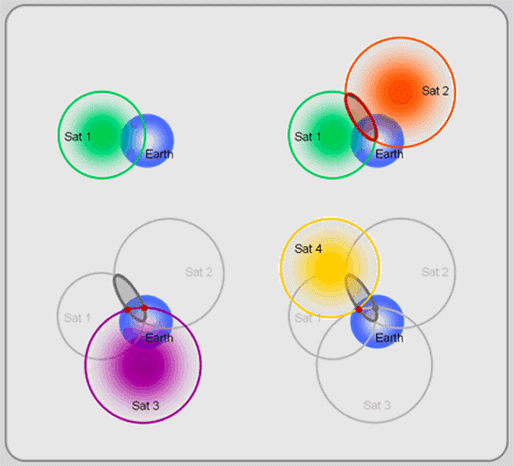
\includegraphics[width=0.40\textwidth]{trilaterate.jpg}
  \caption[GPS trilaterate figure]
   {Figure showing how GPS satellites are used to trilaterate to determine a GPS receivers position. Source: \cite{GISTRILATERATE}}
\end{wrapfigure}
In fields like emergency response, search and rescue, fleet management and even agriculture, it has become a vital tool of utmost importance to everyday operation. Satellite navigation can be found in most new cars and few phones are today sold without an internal GPS receivers. The European Space Agency estimated that there were 2 billion GPS enabled devices by 2012 \cite{ESA}. What started out as a navigation tool for the U.S navy is now used by millions, if not billions of users both civilian and military all over the globe. A common misconception (that is often reinforced by Hollywood action movies) is that the GPS satellites track \textit{you} by communicating with your GPS receiver. It actually works the other way around. You are, with your GPS receiver, tracking a set of satellites in order to establish your own position. At any given time, there are at least 24 GPS satellites each in its own orbit at about 20,372 nautical miles above your head \cite{GPSGOVSS}. In order for a GPS receiver to determine its position and obtain correct time, it will need 4 GPS satellites within line of sight \footnote{The line of sight requirement might seem unreasonable, but by the time the signal has reached earth, is has degraded to a minimum of -160 dBW \cite{NATINT}}.
The method used by your GPS receiver to determine its position is called \textit{trilateration}. 
Trilateration is used in geometry as a process of determining the location (absolute or relative) of point by measuring distance. It is often confused with triangulation which instead of distance, uses angles. Measuring the distance from the GPS satellites to a given position on earth is quite simple when using the equation: 
\begin{equation} Distance = Rate \times Time \end{equation} 
The equation is simple to solve, first we need the rate. In this context, the \textit{rate} is how fast the signals travel. This is equal to the speed of light (299,792,458 m/s). The time the signal has used traveling from the satellite to earth can be obtained by analyzing the signal itself. A simple and slightly inaccurate description is the signal contains a "time stamp" of when the signal was sent. By comparing this time stamp with the current time, one can calculate the age of the signal and therefore how long it has spent traveling. This is explained in greater detail under (\ref{GST}) \cite{GPSGOVTE}.  

\section{Clocks}
\begin{wrapfigure}{c}{0.35\textwidth}
  \centering
  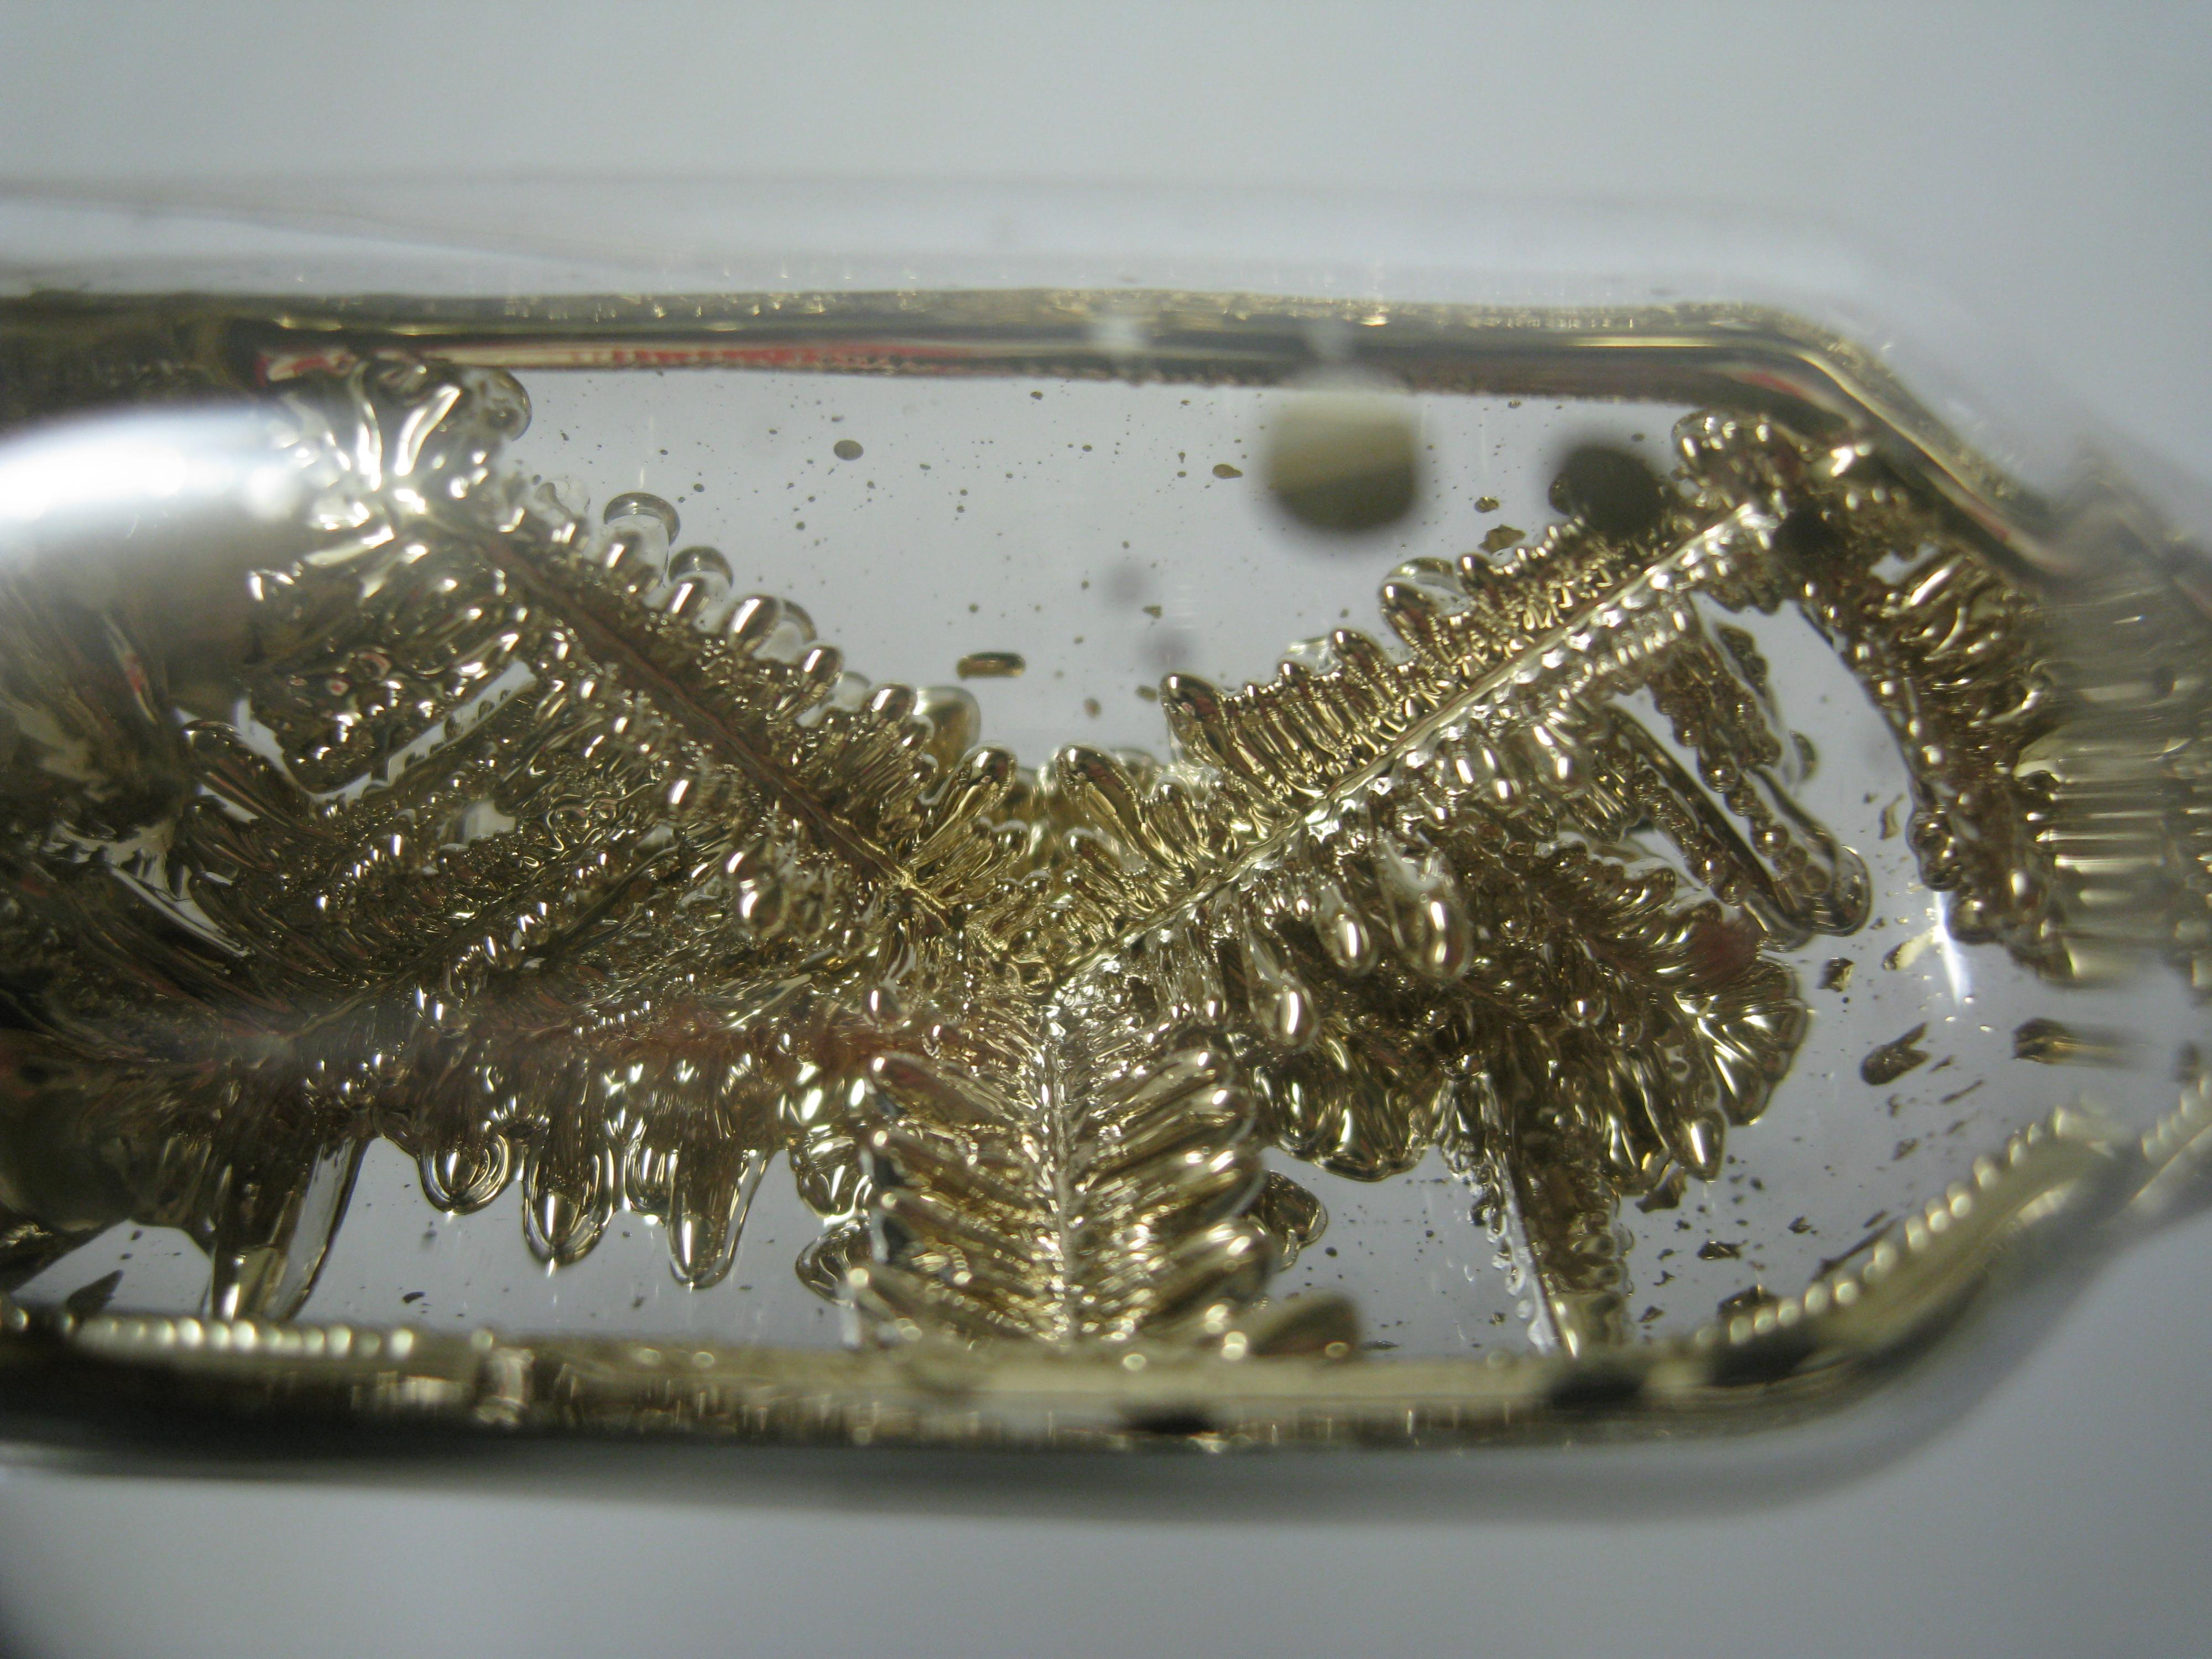
\includegraphics[width=0.30\textwidth]{cscrystals.jpg}
  \caption[Caesium ampule]
   {High pure Caesium crystals in ampule under argon. Source: \cite{DENCES}}
\end{wrapfigure} 
What does a \$10 wristwatch and a \$100 000 atomic clock have in common? They don't stay accurate forever. This phenomena known as \textit{frequency drift}, is when a clock no longer runs at the exact same speed as a reference clock and they drift apart. This property is a result of how they track time. In essence, all clocks work in the same way. They have a part that oscillates, a way to count the number of oscillations and a way to show the count. If we transfer this analogy to the typical "grandfather clock", the pendulum would be the oscillator, the counting mechanism the clockwork and the clock face and dials would be the display. In a typical wristwatch, the oscillator is a quartz crystal powered by a battery. The frequency of which the crystal oscillates is then divided down to a single Hertz by simple electronics. The purity of the crystal is among the decisive factors determining the accuracy of the clock. \cite{CSMG}. Although a completely different beast, the same principles apply to the atomic clock which uses the microwave radiation that electrons in atoms emit when they change energy levels. One of the most commonly used elements in atomic clocks, is \textit{caesium-133}, an isotope of caesium.\footnote{1 second equals 9,192, 631,770 cycles of the Cs-133 transition} \cite{HP}.

\section{GPS signals and Time}\label{GST}
During the introduction of this thesis the properties of GPS as a tool for navigation was made apparent. This is however not the only use of GPS, it is also used for timing. The GPS satellites transmits a \textit{Coarse/Acquisition (C/A)} code and a restricted \textit{Precision (P)} code. The C/A code is freely open for everyone and is transmitted at the L1 carrier frequency (1575.42 MHz) and the P code is transmitted at both L1 and L2 (1227.60 MHz) and is reserved for the military. The C/A code is a 1023 bit pseudo random code that is transmitted at 1.023 Mbit/s, which means it repeats itself every millisecond. Each satellite transmits a different pseudo random code, codes that does not correlate well with each other. This is important because it makes it possible to separate the satellites from each other. The way the receiver calculates its position was briefly mentioned during the introduction and is better explained here. The receiver calculates the distance from itself to the satellites by comparing the pseudo random code received from the satellite with an identical one it generates itself. The receiver "slides" these codes over each other further and further in an attempt to match them up. The signals travel time is determined by how far the codes had to be slided before the matched. This is what is called \textit{Code-phase GPS} and it has got some problems. Since the codes have a wide cycle width, almost a microsecond, there is still a significant uncertainty though the codes match. At the speed of light, a micrFTsecond wrong translates to a roughly 300 meter error in the solved position. What many receivers do is that they start with the code-phase and move on to using measurements based on the carrier frequency. Since the frequency is much higher, the uncertainty withing the match decreases thus increasing the accuracy dramatically. This is whats known as \textit{Carrier-phase GPS}. These signals can be seen as range signals, used to measure distance. This is however not the whole story. The GPS signals also include \textit{navigation message}\label{nav_message} like \textit{ephemeris} as well something called the \textit{almanac}. The ephemeris data orbital information that every GPS satellite in the constellation transmits. This is used by the receiver to calculate the satellites position. The almanac is a state report of the whole constellation. 

Alright, but what about time? We have already established that the key to GPS is measuring the travel time of a radio signal, but considering the consequences of a couple of microseconds of slack when dealing with light-speed, it is really putting some pressure on a GPS receiver's internal clock. As previously mentioned, all your receiver needs to do to find its position in a three dimensional space, is three GPS satellites. If the GPS receivers internal clocks were perfect, the three satellite ranges would intersect at a single point, your position. But in the real world our clocks are everything but perfect. One could use atomic clocks in the receivers but that would make the receivers too expensive (even though chip scale atomic clocks (CSAC) are becoming increasingly affordable \ref{op}) for anyone to buy. The solution is to make a fourth measurement from a fourth satellite. This measurement will not intersect with the first three when using an imperfect clock. The receiver can then try to find a correction factor it can subtract from its timing measurement in order to make the measurements intersect. By doing this, it also brings the receivers clock back to sync with universal time. With the correct time, it can also make correct and precise positioning. \cite{TRIMBLETIME}

\section{GPS time applications}
An example of an application relying on GPS derived time is a PMU (phasor measurement unit). A PMU analyzes the waves on the electrical grid and uses a common time source for synchronization. This synchronization allows for real-time measurements between multiple points in the grid by multiple PMUs. The common time source (and why PMUs are relevant) is often obtained by using GPS. \cite{YLJRNR} The value of such a device is understood clearer by recognizing that the power grid is a complex, interconnected, interdependent network. In other words, errors and abnormalities in one part of the grid will have an effect on operation elsewhere and in some cases lead to whole spread blackouts \cite{EVPMUGA}. GPS time is used in telecommunication to synchronize base stations. The radio spectrum used by cellular phones is limited, making synchronization between base stations important in order to  maintain efficient use of the spectrum. The ability to accurately time-stamp financial transactions is made possible all over the world using GPS and is crucial for traceability and accountability \cite{GPSGOVSSTIME}.

\section{Threat Models and countermeasures}
The threat models and countermeasures presented in this paper are based on the article \textit{Reliable GPS-Based Timing for Power Systems: A Multi-Layered, Multi Receiver}\cite{HengChouGao14}. The only exception is our proposed countermeasure under \ref{op}.
\subsection{Threats}
\subsubsection{Jamming}\label{jam}
By emitting a high-power signal at the frequencies used by GPS satellites, one can interfere with the signals received by the GPS receiver, effectively denying GPS receivers use of these signals. These signals are already weak considering their travel from space. Such an "attack", although effective, is pretty naive and easily recognized by the jammed party. If your equipment is operational and you don't have a signal, you are probably being jammed.

\subsubsection{Signal-level Spoofing}\label{sls}
Signal-level spoofing is when an attacker causes a receiver to loose lock on an authentic GPS signal by overpowering it with a false signal. This can be achieved by using a GPS simulator that matches the authentic signals phase, code delay and encoded data \cite{SGRCOOPMU}. Knowing the signal that the victim is receiving is important in order to successfully spoof it. To anyone with access to the military-grade GPS signals, this is less of an issue since military-grade signals are encrypted and harder to spoof, the civilian frequencies on the other hand are publicly known and readily predictable. Shepard, Humphreys and Fansler (2012)\cite{EVPMUGA} describes in their paper \textit{Evaluation of the Vulnerability of Phasor Measurement Units to GPS Spoofing Attacks}, a way to successfully spoof a GPS signal used by a PMU. They describe how they "introduce" the counterfeit signal to the victim receiver by adjusting the power of the signal below the victim receivers noise floor and then gradually raise it until it surpasses the authentic signals strength. Once the victims receiver locks on, the attacker has gained full control.

\subsubsection{Data-level Spoofing}\label{dls}
In data-level spoofing, the contents (data) of the GPS signal are manipulated. GPS signals include ephemeris data used to solve the positions of each satellite in orbit and also the time and status of the satellite constellation. By altering this data, the receiver solves incorrect velocity, location and most important in this context, clock offset.\cite{SGRCOOPMU}

\subsubsection{Replay spoofing}\label{rs}
Replay spoofing (or \textit{meaconing}\footnote{\textit{Meacon} is portmanteau of \textit{Masking Beacon}}) is a technique where GPS signals are intercepted and rebroadcasted. The rebroadcast can be delayed and used to confuse navigation or to cause delay in applications relying on GPS signals for time.

\subsubsection{Malfunctions}\label{mf}
Just like any tool or device, a GPS receiver is prone to failure. This threat may not be posed by an external party, but is still a threat to normal operation. The ability to differentiate between an attack and a malfunction is important when deciding how to respond to such an event.

\subsection{Countermeasures}
\subsubsection{Monitoring Signal Power}\label{msp} %[C1]
In any kind of attack, jamming or spoofing, a counterfeit signal must overpower the authentic signal in order for the receiver to lock onto it or in the case with jamming, denying access to the authentic signal. By monitoring the strength of the signal and detecting a spike or rise in signal power, a possible attack can be identified. This is a low-cost, low-complexity and independent (in contrast to for example using other receivers as a reference) countermeasure. It is however because of the unpredictable nature of signals, not considered to be a detection confident countermeasure and should therefore only be used along side other countermeasures.\cite{HengChouGao14}

\subsubsection{Checking solved position against known position}\label{cspakp} %[C7]
By checking the position solution against the known position of the receiver, both receiver errors and a replay spoofing attack can be detected. It does however fall short when more sophisticated techniques like Data and Signal-level spoofing ,are used. These kind of attacks when done properly (unless it's done with intention), will not alter the solved position. It is important to note that this is only relevant when only using \textit{one} receiver. If the position solution from multiple receivers deployed in the same area are cross-checked, this countermeasure can still be considered effective. Consider the following scenarios when using 3 receivers:
\begin{itemize}
  \item \textbf{None of the receivers are spoofed:} Each receiver's solved position matches their respective known position. They all solve the same time.
  \item \textbf{One or two receivers are spoofed:} The spoofed receiver(s) solve(s) different time compared to the receiver(s) not being spoofed.
  \item \textbf{All the receivers are spoofed:} As long as they are spoofed by the same spoofer, they will solve the same time but also the same position which again makes it possible to detect the attack.
\end{itemize}
A possible way for an attacker to avoid detection would be to use one spoofer per receiver. These spoofers would need to be synchronized and their signal power fine tuned to make sure that they only spoof their respective receiver. It is believed that such an attack would be too complex and costly to be considered practical. \cite{HengChouGao14}

\subsubsection{Checking time solutions against receiver clock statistics}\label{ctsarcs} %[C8]
By comparing statistics created by monitoring the receiver's clock with the time solution, one can detect spoofing, as well as malfunctions. This is because the time solution is unlikely to be consistent with the statistics in event of an attack. Since this countermeasure relies on the receivers clock which can be described as both unpredictable and stochastic, it should only be used along side other countermeasures.\cite{HengChouGao14}    

\subsubsection{Cross-checking navigation data among receivers}\label{ccndar} %[C5]
When under a data-level spoofing attack , the navigation data is modified. By comparing one GPS receivers navigation data with another, both data-level spoofing and malfunctions can be detected. This countermeasure can also prove useful during jamming attacks because a jammed receiver could use the data from other receivers in the event that is unable to correctly decode navigation, but still able to track satellites. This may enable the receiver to continue operation during an attack. \cite{HengChouGao14}  

\subsubsection{Comparing navigation data and reverse-calculated satellite positions}\label{cndrcsp} %[C6]
The PMU's GPS receivers are never moved and their position is always known. By using their pseudorange measurements, the satellites' positions can be reverse calculated by using trilateration. Since the reverse-calculated positions only match the positions calculated from the navigation data when both pseudorange and navigation data is correct, one can effectively detect replay spoofing and malfunctions. Its also worth noting that this countermeasure increases the difficulty of both signal and data-level spoofing, because it narrows down the possible valid (seemingly) spoofing signals. \cite{HengChouGao14} 

\subsubsection{Cross-correlating P(Y) code}\label{ccpc} %[C2]
This countermeasure assumes two receivers with at least 1 km distance from each other that tracks a signal from a satellite visible to them both. It is also based on the assumption that the encrypted military P(Y) code cannot be forged by a spoofer. The receivers use the C/A code phase and timing relationship to the P(Y) code to obtain two samples from the same time frame of the received P(Y) code and then correlate the two samples. Even though the samples will be encrypted, noisy and perhaps distorted by narrow-band RF front-ends, a high correlation peak should be created when a cross-correlation is conducted as long as the receivers are not spoofed. A key conclusion of the research made by L. Heng (2013) as referenced by L. Heng \textit{et alia} (2014) was that the probability of detection errors using this method decreased exponentially with the length of the samples made from the P(Y) code and the number of receivers used as reference. This method has therefore proved itself effective against spoofing attacks, but ineffective against replay spoofing because the rebroadcast uses authentic GPS signals with correct P(Y) code. It is important to note that the implementation of this countermeasure relies on the GPS receiver's ability to output baseband samples and these samples ability to be transfered over a data network. Because the sampling rate of the samples are fairly high, it is recommended that the spoofing detection is done periodically instead of continuously. \cite{HengChouGao14}  

\subsubsection{Position Aided (PIA) Tracking loops}\label{ptl} %[C3]
\textit{Vector tracking} is a receiver architecture that combine the tasks of signal tracking and position/velocity estimation into one algorithm. This is a contrast to the traditional way where the tracking methods track satellites independently as well as the position/velocity solution independently. Even though this requires more computing power, it increases immunity to interference and jamming. The vector tracking is aided by the fact the we know the PMU GPS receivers true location. The tracking robustness can be further improved by using a Kalman filter. Since a PMU and its GPS receiver remain stationary, the parameters of the tracking loops can be chosen to narrow the loop filter bandwidth which reduces noise and the effective radius of a potential jamming attack. Replay spoofing attacks will also fail since the PIA vector tracking depends on the knowledge of the GPS receivers true position. In the event of such an attack, the result would be that the vector tracking will fail to function. \cite{HengChouGao14}  

\subsubsection{Multi-receiver tracking loops}\label{mrtl}
Building on the idea from \textit{PIA Tracking loops} one can benefit from the networked nature of the GPS-timed PMU. In a multi-receiver vector tracking loop, many receivers process information in collaboration. A key conclusion of the research made by A. Soloviev \textit{et alia} as referenced by L. Heng \textit{et alia} (2014) showed that acquisition and tracking performance under low signal-to-noise ratio conditions was improved under multi-receiver signal accumulation. Multi-receiver phased arrays also improved the robustness against both jamming (\ref{jam}) and spoofing attacks (\ref{sls},\ref{dls}) by \textit{"Forming beams to satellites and steering nulls in the direction of attacking transmitters"} (L. Heng \textit{et alia} (2014), p.41). In addition to the increased robustness, it increases the ability to detect malfunction. A faulty receiver will usually not be consistent with other correctly functioning receivers. As with the countermeasure based on cross-correlating P(Y) code, this implementation also requires that the GPS receivers are able to output baseband samples. In this implementation, the samples need to be transmitted continuously among the receivers which requires a capable data network such as a typical LAN. \cite{HengChouGao14} 

\newpage
\subsection{Summary}
The table (\ref{tab:threatcounttable}) shows the different threat models and the effect of the countermeasures discussed.

\begin{savenotes}
\begin{table}[h]
  \caption{The table shows the effectiveness of the covered countermeasures against threat models.}
  \begin{tabular}{|l|c|c|c|c|c|} \hline
  \multicolumn{1}{|c|}{\multirow{2}{*}{Counter Measures}} &
  \multicolumn{5}{c|}{Threat Models} \\ \cline{2-6} 
    \multicolumn{1}{|c|}{} & 
    \multicolumn{1}{l|}{\vtop{\hbox{\strut JAM\footnote{Jamming (\ref{jam})}}}} &
    \multicolumn{1}{l|}{\vtop{\hbox{\strut SLS\footnote{Signal-level Spoofing (\ref{sls}) }}}} & 
    \multicolumn{1}{r|}{\vtop{\hbox{\strut DLS\footnote{Data-level Spoofing (\ref{dls}) }}}} & 
    \multicolumn{1}{l|}{\vtop{\hbox{\strut RS\footnote{Replay Spoofing (\ref{rs}) }}}} & 
    \multicolumn{1}{l|}{\vtop{\hbox{\strut MF\footnote{Malfunctions (\ref{mf}) }}}}\\ 
    \hline
    Monitoring Signal Power      (\ref{msp})        & \cellcolor{ineffectivec}N & \cellcolor{effectivec}X & \cellcolor{effectivec}X & \cellcolor{effectivec}X & \cellcolor{ineffectivec}N \\ \hline
    Check pos. solution          (\ref{cspakp})     & \cellcolor{ineffectivec}N & \cellcolor{auxiliryc}Y & \cellcolor{auxiliryc}Y & \cellcolor{auxiliryc}Y & \cellcolor{auxiliryc}Y \\ \hline
    Check time solutions         (\ref{ctsarcs})    & \cellcolor{ineffectivec}N & \cellcolor{effectivec}X & \cellcolor{effectivec}X & \cellcolor{effectivec}X & \cellcolor{effectivec}X \\ \hline
    Checking nav. data           (\ref{ccndar})     & \cellcolor{effectivec}X & \cellcolor{ineffectivec}N & \cellcolor{auxiliryc}Y & \cellcolor{ineffectivec}N & \cellcolor{auxiliryc}Y \\ \hline
    Reverse calculated sat. pos. (\ref{cndrcsp})    & \cellcolor{ineffectivec}N & \cellcolor{effectivec}X & \cellcolor{effectivec}X & \cellcolor{auxiliryc}Y & \cellcolor{auxiliryc}Y \\ \hline
    Cross-correlating P(Y)       (\ref{ccpc})       & \cellcolor{ineffectivec}N & \cellcolor{auxiliryc}Y & \cellcolor{auxiliryc}Y & \cellcolor{ineffectivec}N & \cellcolor{ineffectivec}N \\ \hline
    PIA TL                       (\ref{ptl})        & \cellcolor{auxiliryc}Y & \cellcolor{ineffectivec}N & \cellcolor{ineffectivec}N & \cellcolor{auxiliryc}Y & \cellcolor{ineffectivec}N \\ \hline
    Multi-receiver TL            (\ref{mrtl})       & \cellcolor{auxiliryc}Y & \cellcolor{effectivec}X & \cellcolor{effectivec}X & \cellcolor{effectivec}X & \cellcolor{effectivec}X \\ \hline
    %CSAC SMACC                   (\ref{op})         & \cellcolor{auxiliryc}Y & \cellcolor{auxiliryc}Y & \cellcolor{auxiliryc}Y & \cellcolor{auxiliryc}Y & \cellcolor{auxiliryc}Y \\ \hline
  \end{tabular}
  \label{tab:threatcounttable}
\end{table}
\end{savenotes} 

 \begin{table}[h]
    \caption{Legend for table (\ref{tab:threatcounttable}) }
    \begin{tabular}{|c|c|c|c|c|c|}
    \hline
    \cellcolor{auxiliryc}Y & Effective & \cellcolor{ineffectivec}N & Ineffective & \cellcolor{effectivec}X & Auxiliary \\ \hline
    \end{tabular}
  \end{table} 

\newpage
\section{Benchmark clock spoofing attack}\label{benchmark_spoofer}
In 2012 a team from The University of Texas at Austin published a paper describing \textit{The Civil GPS Spoofer}. It was a GPS spoofer and the first of its kind. The Cilvil GPS spoofer was able to precisely align both the C/A codes and navigation data in a counterfeit signal, with those of an authentic GPS signal. The alignment capability allowed for sophisticated spoofing attacks that was hard to detect. The spoofer was implemented in software-defined radio with a digital signal processor. The user could control the fake GPS signal, specifying both navigation and timing. By tracking an acquiring GPS signals and calculating navigation data, it could produce up to 14 spoofed L1 C/A signals by performing real-time prediction of the pseudo random C/A codes. Key features of the time spoofing attack: 
\begin{itemize}
  \item Seamless takeover: GPS spoofer tricks target into locking on to a replica of the authentic GPS signal, without loss of GPS lock or change in reported position. 
  \item Once target is locked on to spoofer signal, the attacker manipulates the apparent time of the target GPS clock. 
  \item Low quality internal clocks enable aggressive manipulation of GPS clock timing, rapidly resulting in large apparent timing errors.
\end{itemize} 
The sophistication of this spoofing attack is in part due to it's technical complexity, but more importantly due to the demonstrated result: The attacked GPS controlled clock had no way to detect that it was being fed false GPS signals. The study is targeted to the use of timing to phasor measurement units used in the monitoring and control of power grid transmission lines. The aggressive manipulation of timing may have caused the malicious shutdown of transmission lines within a few minutes after the onset of the attack. The team tested the spoofer against a wide variety of applications using the civilian receivers, and they were always successful \cite{EVPMUGA}. When designing spoof proof GPS systems, the Civil GPS spoofer can be considered a benchmark reference threat. 